\documentclass[12pt,a4paper]{article}
\usepackage[utf8]{inputenc} % inutile avec XeLaTeX/LuaLaTeX
\usepackage[T1]{fontenc}
\usepackage{amsmath,amssymb,mathrsfs,tikz,times,pifont}
\usepackage{enumitem}
\usepackage{multicol}
\usepackage{lmodern}
\newcommand\circitem[1]{%
\tikz[baseline=(char.base)]{
\node[circle,draw=gray, fill=red!55,
minimum size=1.2em,inner sep=0] (char) {#1};}}
\newcommand\boxitem[1]{%
\tikz[baseline=(char.base)]{
\node[fill=cyan,
minimum size=1.2em,inner sep=0] (char) {#1};}}
\setlist[enumerate,1]{label=\protect\circitem{\arabic*}}
\setlist[enumerate,2]{label=\protect\boxitem{\alph*}}
\everymath{\displaystyle}
\usepackage[left=1cm,right=1cm,top=1cm,bottom=1.7cm]{geometry}
\usepackage[colorlinks=true, linkcolor=blue, urlcolor=blue, citecolor=blue]{hyperref}
\usepackage{array,multirow}
\usepackage[most]{tcolorbox}
\usepackage{varwidth}
\usepackage{float}
\tcbuselibrary{skins,hooks}
\usetikzlibrary{patterns}

\newtcolorbox{exa}[2][]{enhanced,breakable,before skip=2mm,after skip=5mm,
colback=yellow!20!white,colframe=black!20!blue,boxrule=0.5mm,
attach boxed title to top left ={xshift=0.6cm,yshift*=1mm-\tcboxedtitleheight},
fonttitle=\bfseries,
title={#2},#1,
boxed title style={frame code={
\path[fill=tcbcolback!30!black]
([yshift=-1mm,xshift=-1mm]frame.north west)
arc[start angle=0,end angle=180,radius=1mm]
([yshift=-1mm,xshift=1mm]frame.north east)
arc[start angle=180,end angle=0,radius=1mm];
\path[left color=tcbcolback!60!black,right color = tcbcolback!60!black,
middle color = tcbcolback!80!black]
([xshift=-2mm]frame.north west) -- ([xshift=2mm]frame.north east)
[rounded corners=1mm]-- ([xshift=1mm,yshift=-1mm]frame.north east)
-- (frame.south east) -- (frame.south west)
-- ([xshift=-1mm,yshift=-1mm]frame.north west)
[sharp corners]-- cycle;
},interior engine=empty,
},interior style={top color=yellow!5}}

\usepackage{fancyhdr}
\usepackage{eso-pic}
\usepackage{tkz-tab}
\AddToShipoutPicture{
    \AtTextCenter{%
        \makebox[0pt]{\rotatebox{80}{\textcolor[gray]{0.7}{\fontsize{5cm}{5cm}\selectfont PGB}}}
    }
}

\usepackage{verbatim}

\usepackage{color,soul}

\usepackage{amsmath}
\usepackage{amsfonts}
\usepackage{amssymb}
\usepackage{systeme}
\usepackage{tkz-tab}
\usepackage{tikz}
\usetikzlibrary{arrows}
\newcounter{exemple} % Compteur pour les questions

% Définir la commande pour afficher une question numérotée
\newcommand{\exemple}{%
  \refstepcounter{exemple}%
  \textbf{\textcolor{green}{Exemple \theexemple :}} \ignorespaces
}
%---------------------------------------
\definecolor{myorange}{rgb}{1.0, 0.8, 0.0}

% Définir un compteur pour les exercices d'application
\newcounter{exerciceapp}

% Définir la commande pour afficher un exercice d'application numéroté
\newcommand{\exerciceapp}{%
  \refstepcounter{exerciceapp}%
  \textbf{\textcolor{myorange}{Exercice d'application \theexerciceapp :}} \ignorespaces
}
%--------------------------------------
% Définir un compteur pour les exercices d'application
\newcounter{correction}

% Définir la commande pour afficher un correction exercice d'application numéroté
\newcommand{\correction}{%
  \refstepcounter{correction}%
  \textbf{\textcolor{myorange}{Correction \thecorrection :}} \ignorespaces
}
%--------------------------------------
% Commande pour ajouter du texte en arrière-plan
\usepackage{fancyhdr}
\usepackage{eso-pic}
%\usepackage{tkz-tab}
\AddToShipoutPicture{
    \AtTextCenter{%
        \makebox[0pt]{\rotatebox{80}{\textcolor[gray]{0.7}{\fontsize{5cm}{5cm}\selectfont PGB}}}
    }
}
%This command takes a colour as an optional argument; the default colour is black.
\usetikzlibrary{shapes.geometric,fit}
\newcommand{\myul}[2][black]{\setulcolor{#1}\ul{#2}\setulcolor{black}}
\newcommand\tab[1][1cm]{\hspace*{#1}}

\begin{document}
% En-tête personnalisée
\begin{center}
    \Large\textbf{\underline{\textcolor{red}{Calcul Intégral Ts2}}}\\[-0.1cm]
    \normalsize\textbf{Prof : M. BA} \hfill \textbf{Classe : TS2}\\[-0.1cm]
    \textbf{Année scolaire : 2024 -- 2025}
\end{center}

\section*{\underline{\textbf{\textcolor{red}{I. Intégrale d'une fonction continue: }}}}
\subsection*{\underline{\textbf{\textcolor{red}{1.Introduction :}}}}

Soit \( f \) une fonction continue sur un intervalle \( I \),\( F \) et \( G \) 2 primitives de \( f \) sur \( I \), \( a \) et \( b  \) deux éléments de I. On sait qu'il existe un nombre réel $c$ tel que :$\forall x\in I$, 
 \( G(x) = F(x) + c \)

\underline{\( 
\begin{cases}
G(a) = F(a) + c\\
G(b) = F(b) + c
\end{cases}
\)}

\(
\quad G(b) - G(a) = F(b) - F(a)
\)

Le nombre réel \( F(b) - F(a) \) est donc indépendant de la primitive \( f \) choisie

\subsection*{\underline{\textbf{\textcolor{red}{2.Définition :}}}}

Soit \( f \) une fonction continue sur un intervalle \( I \).
En appelle intégrale de \( a \) à \( b \) de \( f \) le nombre réel \( F(b) - F(a) \) où \( F \) est une primitive de \( f \) sur \( I \) on note :

\[
F(b) - F(a) = \int_{a}^{b} f(x) \, dx = \left[ F(x) \right]_{a}^{b}
\]

\begin{itemize}
    \item \( \int_a^b f(x) \, dx \) se lit ``intégrale ou somme  de $a$ à $b$ de $f(x)dx$''.
    \item \( \left[ F(x) \right]_a^b \) se lit ``\( F(x) \) pris entre \( a \) et \( b \)''.
    \item \( a \) et \( b \) sont les bornes de l'intégrale \( \int_a^b f(x) \, dx \)
        \item Dans l'écriture \( \int_a^b f(x) \, dx \) On peut remplaçer \( x \) par toute autre lettre (sauf \( a \) et \( b \)) on écrit \( \int_a^b f(t) \, dt \) ou \( \int_a^b f(s) \, ds \) ; \( x \) est appelé variable muette.
\end{itemize}
\newpage
\section*{\textbf{\textcolor{red}{Exemple 1}}}

\[
f(x) = x^2, \quad F(x) = \frac{1}{3} x^3
\]

\[
\begin{aligned}
\int_1^2 f(x) \, dx &= \left[ \frac{1}{3} x^3 \right]_1^2 \\
&= \frac{1}{3} \left[ 2^3 - 1^3 \right] \\
&= \frac{1}{3} \left[ 8 - 1 \right] \\
&= \frac{7}{3}
\end{aligned}
\]

\[\boxed{\int_1^2 f(x) \, dx=\frac{7}{3}} \]

\section*{\textbf{\textcolor{red}{Exemple 2}}}

\[
f(x) = \cos x, \quad F(x) = \sin x
\]

\[
\begin{aligned}
\int_0^{\frac{\pi}{4}} \cos x \, dx &= \left[ \sin x \right]_0^{\frac{\pi}{4}} \\
&= \sin \left( \frac{\pi}{4} \right) - \sin(0) \\
&= \frac{\sqrt{2}}{2} - 0 \\
&= \frac{\sqrt{2}}{2}
\end{aligned}
\]

\[\boxed{\int_0^{\frac{\pi}{4}} \cos x \, dx = \frac{\sqrt{2}}{2}} \]

\section*{\textbf{\textcolor{red}{Propriété 1 }}}
Soit \( f \) une fonction continue sur un intervalle \( I \), \( a \) et \( b \) deux élément de \( I \). On a
\[
\int_a^a f(x) \, dx = 0 \quad;\quad \quad \int_a^b f(x) \, dx = - \int_b^a f(x) \, dx
\]

En effet :

\[
\int_a^b f(x) \, dx = \left[ F(x) \right]_a^b = F(b) - F(a) = 0
\]

\[
\int_a^b f(x) \, dx = \left[ P(x) \right]_a^b = F(b) - F(a) = - \left( P(b) - P(a) \right)=-\int_b^a f(x) \, dx
\]

\subsection*{\underline{\textbf{\textcolor{red}{3. Intégrale et Primitive :}}}}

Soit \( f \) une fonction continue sur \( I \) (intervalle), \( a \in I \), \( F \) primitive de \( f \) sur \( I \), telle que \( F'(x) = f(x) \), et \( F(a) = 0 \). \(F(x) = \int_a^x f(t) \, dt \)

En effet:

\[
\int_a^x f(t) \, dt = F(x) - F(a) = F(x) - 0
\]

\subsection*{\underline{\textbf{\textcolor{red}{4. Interprétation graphique de l'intégrale :}}}}

Soit \( f \) une fonction continue et \textcolor{red}{positive} sur un intervalle \( I \), \( (Cf) \) sa courbe représentative, \( a \) et \( b \in I \) avec \( a < b \).

\(
\int_a^b f(x) \, dx \text{ est l'aire (en unité d'aire) du domaine D délimité par la courbe \( (Cf) \),}\\ \text{l'axe des abscisses \( (OI) \) et les droites d'équation \( x = a \), \( x = b \).}
\)

\(
\text{ Ce domaine est aussi l'ensemble des points $M\begin{pmatrix} x \\ y \end{pmatrix}$  tel que}:
\begin{cases}
a \leq x \leq b \\
0 \leq y \leq f(x)
\end{cases}
\)

\[\text{Ainsi,en notant A(D), aire du domaine et u.a unité d'aire, on a: }
A(D)=\int_a^b f(x) \, dx .u.a 
\]

\begin{center}
   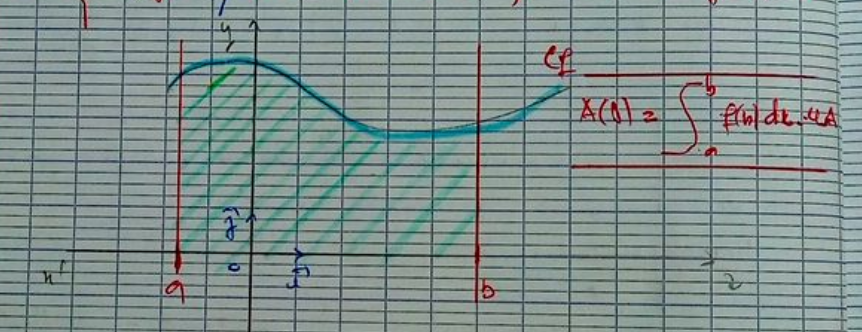
\includegraphics[scale=0.5]{Screenshot from 2025-04-26 23-30-27.png}
\end{center}

\section*{\textbf{\textcolor{red}{Remarque}}}
Si \( f \) une fonction continue et \textcolor{red}{négative} sur \([a,b]\). La symétrie orthogonale d'axe \( (OI) \) transforme la courbe \(\mathcal{C}_f\) en celle de \( \mathcal{C}'_{-f} \) de f.

Le domaine \( D \) est tranformé en un domaine \( D' \) de meme aire

\( \text{on a :} A(D)=A(D')=\int_a^b -f(x) \, dx .u.a  \)
\begin{center}
   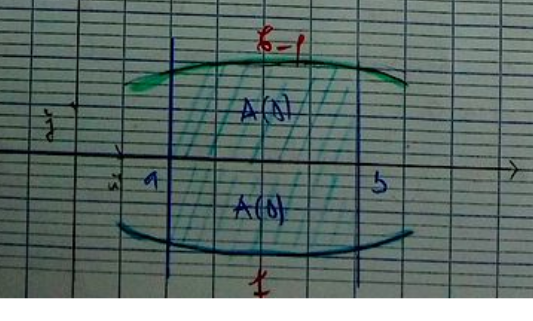
\includegraphics[scale=0.5]{Screenshot from 2025-04-27 00-00-46.png}
\end{center}

\section*{\textbf{\textcolor{red}{Exemple 3}}}

L'unité graphique est $2cm$ sur chaque axes.

Calculer l'aire, en $cm^{2}$ de l'ensemble D des points M(x,y) tels que :

 \(-\frac{\pi}{2}\leq x \leq \frac{\pi}{2} \) et \( 0\leq y \leq \cos x \)

\section*{\textbf{\textcolor{red}{Solution 3}}}

La fonctionFonction cosinus est continue et positif sur \( \left[ -\frac{\pi}{2}, \frac{\pi}{2}\right]  \)

On a : $\int_{-\frac{\pi}{2}}^{\frac{\pi}{2}}dx.u.a$ avec $u.a = 2cm \times 2cm=4cm^{2}$

\section*{\textbf{\textcolor{red}{Exemple 4}}}

La courbe ci-dessous est la representation graphique de la fonction $f(x)=x^{2}-1$ .Calculer l'aire du domaine colorié.

\begin{center}
   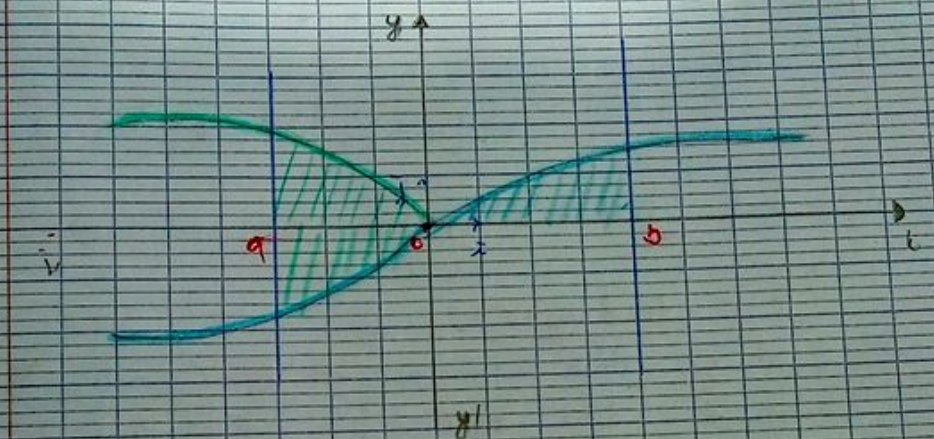
\includegraphics[scale=0.5]{Screenshot from 2025-04-27 08-29-47.png}
\end{center}  

\section*{\textbf{\textcolor{red}{Exemple 3}}}

$f(x)=x^{2}-1$

          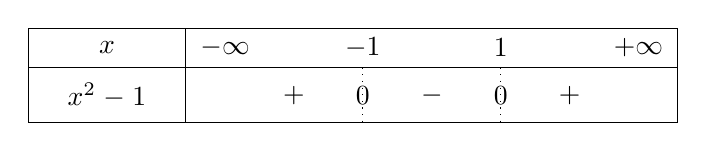
\begin{tikzpicture}[node style/.style={fill opacity=0,text opacity=1}]
              \tkzTabInit[espcl=1.75]{$x$/.5,$x^{2}-1$/.7}{$-\infty$,$-1$,$1$,$+\infty$}
              \tkzTabLine{,+,z,-,z,+}
          \end{tikzpicture}

\begin{center}
   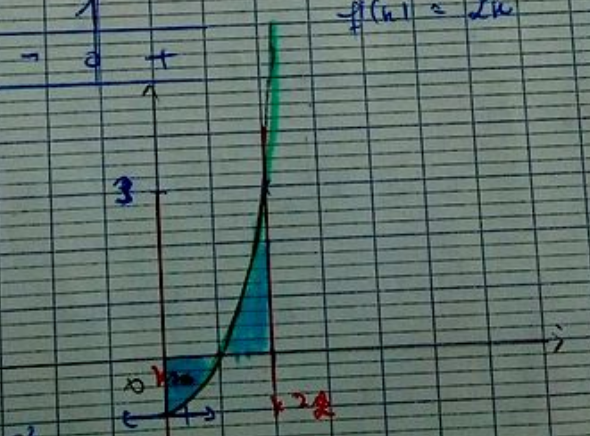
\includegraphics[scale=0.5]{Screenshot from 2025-04-27 08-33-05.png}
\end{center}
\(
\begin{aligned}
A(D) &= \left( \int_0^1 -f(x) \, dx + \int_1^2 f(x) \, dx \right) u.A\\
		 &= \left( \int_0^1 -(x^{2}-1) \, dx + \int_1^2 (x^{2}-1) \, dx \right) u.A\\
		 &=\cdots\\
		 &=2cm^{2}
\end{aligned}
\)  

\[\boxed{A(D)=2cm^{2}}\]   

\section*{\textbf{\textcolor{red}{5.Propriété algébrique de l'intégrale}}}
\subsection*{\textbf{\textcolor{red}{a.Relation de Chasles}}}

Si  \( f \) continue sur un intervalle  \( I \), $a$, $b$ et $c$ trois élément de $K$.

On a:

\[
\int_a^c f(x) \, dx = \int_a^b f(x) \, dx + \int_b^c f(x) \, dx
\]

%\[
%A(D) = \int_a^b -f(x) \, dx.u.A + \int_b^c f(x) \, dx.u.A
%\]

\textbf{Preuve}

\textbf{Interprétation graphique de la relation de Chasles}Voire Ciam pas 298 section 1.2  

\subsubsection*{\underline{\textbf{\textcolor{red}{Exemples}}}}

\(
\begin{aligned}
\int_{-\frac{\pi}{2}}^{\frac{\pi}{2}} \left| \sin(t) \right| \, dt &= \int_{-\frac{\pi}{2}}^{0} -\sin(t) \, dt + \int_{0}^{\frac{\pi}{2}} \sin(t) \, dt\\
&= -\left[\cos(t) \right]_{-\frac{\pi}{2}}^{0} + \left[ \cos(t) \right]_{0}^{\frac{\pi}{2}}\\
&=1+1\\
&=2
\end{aligned}
\)

\( \int_{-\frac{\pi}{2}}^{\frac{\pi}{2}} \left| \sin(t) \right| \, dt = 2 \)

\subsubsection*{\underline{\textbf{\textcolor{red}{b.Linéarité de l'intégrale}}}}

Soit \( f \) et \( g \) deux fonctions continues sur \( I \). 

\( \alpha, \beta \) deux réels,  \( a, b \in I \).

On a:

\[
\boxed{\int_a^b \left( \alpha f + \beta g \right)(x) \, dx = \alpha \int_a^b f(x) \, dx + \beta \int_a^b g(x) \, dx}
\]

\section*{\underline{\textbf{\textcolor{red}{Exemples}}}}
Calculer les intégrales suivantes
\[ \int_0^{\frac{\pi}{4}}\cos^{2}(t)dt\]
\section*{\underline{\textbf{\textcolor{red}{Solution}}}}
\( 
\begin{aligned} 
\int_0^{\frac{\pi}{4}}\cos^{2}(t)dt &=\int_0^{\frac{\pi}{4}}\frac{1+\cos(2t)}{2}dt \\
&=\frac{1}{2}\int_0^{\frac{\pi}{4}}1+\cos(2t)dt \\
&=\frac{1}{2}\int_0^{\frac{\pi}{4}}1+\frac{1}{2}\int_0^{\frac{\pi}{4}}\cos(2t)dt \\
\end{aligned}
\)
\subsection*{\underline{\textbf{\textcolor{red}{6.Signe de l'intégrale:}}}}
i)Soit $f$ une fonction continue sur $I$, $a$ et $b\in I$  $(a<b)$
\begin{itemize}
\item si $f>0$ sur $[a,b]$ alors $\int_a^b f(x)dx \geq 0$
\item si $f<0$ sur $[a,b]$ alors $\int_a^b f(x)dx \leq 0$
\end{itemize}
ii)Soit $f$ et $g$ deux fonctions continues sur $I$, $a$ et $b\in I$  $(a<b)$
\begin{itemize}
\item Si $f \leq g$, $\forall x \in[a,b]$ alors $ \int_a^b f(x)dx \leq \int_a^b g(x)dx$
\end{itemize}
\section*{\underline{\textbf{\textcolor{red}{Exemples}}}}

\subsection*{\underline{\textbf{\textcolor{red}{Remarque :}}}}

Soit \( f \) une fonction continue sur \( I \), \( a \) et \( b \in I \), tel que \( a \leq b \).

On a: \( -|f| \leq |f| \leq |f| \text{ sur } [a ; b] ; \text{on en déduit que} : \left| \int_a^b f(x) \, dx \right| \leq \int_a^b |f(x)| \, dx\)

\subsection*{\underline{\textbf{\textcolor{red}{7. Inégalité de la moyenne :}}}}

\textbf{i)} Soit \( f \) une fonction continue sur \( I \) (intervalle) \( a \) et \( b \in I \)

Si \( m \) et \( M \) sont deux nombres réels tels que \( x \in [a, b] \) \( m \leq f(x) \leq M \),  

\[
\textbf{alors }m (b - a) \leq \int_a^b f(x) \, dx \leq M(b - a)
\]  
\textbf{ii)} Soit \( f \) une fonction continue sur un intervalle \( I \) tel que \( a \leq b \in I \).

Si  \( M \) deux réels tels que \(|f(x)| \leq M, \quad \forall x \in [a,b]\)

On en déduit :

\[
\left| \int_a^b f(x) \, dx \right| \leq M (b-a)
\]

\subsection*{\underline{\textbf{\textcolor{red}{8. Valeur moyenne d'une fonction :}}}}

Soit \( f \) une fonction continue sur un intervalle \( [a, b] \), on appelle valeur moyenne de \( f \) sur \( [a, b] \) le nombre réel \( u \) défini par :

\[
u = \frac{1}{b - a} \int_a^b f(x) \, dx
\]
\section*{\underline{\textbf{\textcolor{red}{II. Techniques de calcul intégral}}}}

\subsubsection*{\underline{\textcolor{red}{1. Primitives usuelles :}}}
Le tableau suivant reprend quelques résultats concernant les primitives, vus dans les chapitres précédents. Dans ce tableau, \( u \) désigne une fonction dérivable sur un intervalle \( K \), \( v \) une fonction dérivable sur un intervalle contenant \( u(K) \) et \( \alpha \) un nombre réel différent de \( -1 \).

\begin{tabular}{|c|c|c|c|c|}
\hline
\textbf{Fonction} & \( \frac{u'}{u} \) & \( u' e^u \) & \( u' u^\alpha \) & \( u' \cdot v' \circ u \) \\
\hline
\textbf{Primitive} & \( \ln |u| \) & \( e^u \) & \( \frac{1}{\alpha + 1} u^{\alpha + 1} \) & \( v \circ u \) \\
\hline
\textbf{Commentaires} & \( u \neq 0 \) sur \( K \) & - & \( u > 0 \) sur \( K \) & - \\
\hline
\end{tabular}

\subsection*{Examples}

\begin{itemize}
    \item \( \int_0^1 \left( t^3 + 2t + 1 \right) \, dt = \left[ \frac{t^4}{4} + t^2 + t \right]_0^1 = \frac{9}{4} \)
    
    \item \( \int_0^{\frac{\pi}{4}} \sin \left( 2t + \frac{\pi}{2} \right) \, dt = \left[ -\frac{1}{2} \cos \left( 2t + \frac{\pi}{2} \right) \right]_0^{\frac{\pi}{4}} = \frac{1}{2} \)
    
    \item \( \int_0^{\frac{1}{2}} \frac{2t}{t^2 - 1} \, dt = \left[ \ln |t^2 - 1| \right]_0^{\frac{1}{2}} = \ln \frac{3}{4} \)
    
    \item \( \int_0^{\frac{\pi}{2}} \cos t \, e^{\sin t} \, dt = \left[ e^{\sin t} \right]_0^{\frac{\pi}{2}} = e - 1 \)
\end{itemize}

\subsubsection*{\underline{\textcolor{red}{2. Intégration par parties :}}}
Soit \( u \) et \( v \) deux fonctions dérivables sur un intervalle \( K \) telles que les dérivées \( u' \) et \( v' \) sont continues sur \( K \), \( a \) et \( b \) deux éléments de \( K \).

On a :

\[
\int_a^b u(t) v'(t) \, dt = \left[ u(t) v(t) \right]_a^b - \int_a^b u'(t) v(t) \, dt
\]

\subsection*{Examples}

\begin{itemize}
    \item Calculer : \( \int_1^2 \ln t \, dt \).
    
    Posons : \( u(t) = \ln t \) et \( v'(t) = 1 \).
    
    On a : \( u'(t) = \frac{1}{t} \) ; choisissons : \( v(t) = t \).
    
    \( u' \) et \( v' \) sont continues sur \( [1 ; 2] \).
    
    Donc :
    \[
    \int_1^2 \ln t \, dt = \left[ t \ln t \right]_1^2 - \int_1^2 dt
    \]
    \[
    = \left[ t \ln t \right]_1^2 - \left[ t \right]_1^2
    \]
    \[
    = \left[ 2 \ln 2 - 2 \right] - \left[ 1 \ln 1 - 1 \right] = 2 \ln 2 - 1
    \]
    
    \item Calculer : \( \int_0^{\frac{\pi}{2}} t \cos t \, dt \).
    
    Posons : \( u(t) = t \) et \( v'(t) = \cos t \).
    
    On a : \( u'(t) = 1 \) ; choisissons : \( v(t) = \sin t \).
    
    \( u' \) et \( v' \) sont continues sur \( [0 ; \frac{\pi}{2}] \).
    
    Donc :
    \[
    \int_0^{\frac{\pi}{2}} t \cos t \, dt = \left[ t \sin t \right]_0^{\frac{\pi}{2}} - \int_0^{\frac{\pi}{2}} \sin t \, dt
    \]
    \[
    = \left[ t \sin t \right]_0^{\frac{\pi}{2}} - \left[ - \cos t \right]_0^{\frac{\pi}{2}}
    \]
    \[
    = \left[ \frac{\pi}{2} \sin \frac{\pi}{2} - 0 \right] - \left[ - \cos \frac{\pi}{2} + \cos 0 \right]
    \]
    \[
    = \left[ \frac{\pi}{2} \times 1 \right] - \left[ - 0 + 1 \right] = \frac{\pi}{2} - 1
    \]
\end{itemize}

\subsubsection*{\underline{\textcolor{red}{3. Intégration de fonctions paires, impaires, périodiques :}}}
\subsubsection*{\underline{\textcolor{red}{Propriété 1 :}}}
Soit \(f\) une fonction continue sur un intervalle \(I\) symétrique par rapport à \(0\).

\( \forall \alpha \in I \), on a:

\begin{itemize}
    \item Si \(f\) est paire, \( \int_{-\alpha}^{\alpha}f(x)dx = 2 \int_{0}^{\alpha}f(x)dx \)
    \item Si \(f\) est impaire, \( \int_{-\alpha}^{\alpha}f(x)dx =  0 \)
\end{itemize}
\subsection*{Examples}
CIAM
\subsubsection*{\underline{\textcolor{red}{Propriété 2 :}}}
Soit \(f\) une fonction continue sur \( \mathbb{R} \) et périodique, de période \(p\).

Pour tous nombres réel \(a\) et \(b\), on a:

\begin{itemize}
    \item Si \(f\) est paire, \( \int_{a+p}^{b+p}f(x)dx = \int_{a}^{b}f(x)dx \)
    \item Si \(f\) est impaire, \( \int_{a}^{a+p}f(x)dx =  \int_{0}^{p}f(x)dx = 0 \)
\end{itemize}
\subsection*{Examples}
CIAM
\section*{\underline{\textbf{\textcolor{red}{III. Application du calcul intégral}}}}
\subsubsection*{\underline{\textcolor{red}{Propriété :}}}
Soit \(f\) et \(g\) deux fonctions continues sur un intervalle \(I\), \( (\mathcal{C}_f) \) et \( (\mathcal{C}_g) \) leurs réprésentations graphiques respectives \(a\) et \(b\) deux éléments de \(I\) (\(a<b\))
Lorsque \(f \leq g\) sur \( [a;b] \), l'aire du domaine \(D\) délimité par \( (\mathcal{C}_f) \), \( (\mathcal{C}_g) \) et les droites d'équations \( x=a \) et \( x=b \) est: \(\mathcal{A}(D)=\int_{a}^{b} [g(x)-g(x)]dx \)

\textbf{Voir dessin}
\subsection*{Examples}
CIAM
\end{document}